%% LyX 2.2.2 created this file.  For more info, see http://www.lyx.org/.
%% Do not edit unless you really know what you are doing.
\documentclass[twoside,english]{extreport}
\usepackage[T1]{fontenc}
\usepackage[latin9]{inputenc}
\usepackage[letterpaper]{geometry}
\geometry{verbose,tmargin=4cm,bmargin=3cm,lmargin=2cm,rmargin=2cm,headheight=1cm,headsep=0.5cm,footskip=1cm}
\setcounter{secnumdepth}{3}
\setcounter{tocdepth}{3}
\usepackage{color}
\definecolor{page_backgroundcolor}{rgb}{1, 1, 1}
\pagecolor{page_backgroundcolor}
\definecolor{document_fontcolor}{rgb}{0, 0, 0}
\color{document_fontcolor}
\usepackage{babel}
\usepackage{float}
\usepackage{amsmath}
\usepackage{graphicx}
\usepackage[unicode=true,pdfusetitle,
 bookmarks=true,bookmarksnumbered=false,bookmarksopen=false,
 breaklinks=false,pdfborder={0 0 1},backref=false,colorlinks=true]
 {hyperref}
\usepackage{breakurl}

\makeatletter
%%%%%%%%%%%%%%%%%%%%%%%%%%%%%% Textclass specific LaTeX commands.
\numberwithin{equation}{section}
\numberwithin{figure}{section}

\makeatother

\begin{document}

\title{\textbf{Dynamics and Control Of Spacecraft}\\
\textbf{Astrosat Controller Design}}

\author{Kavita Sivaraman - AE16M006 \\
Prem Sagar S - AE14B021\\
Rishi - AE17D402\\
Daniel Satke - AE17F010\\
Abdul Azeez - AE14B028}
\maketitle

\chapter{Kinematics and Dynamics of Astrosat}

\section{Introduction}

We are planning to design a preliminary attitude control system for
ASTROSAT satellite. Since this satellite is an inertial pointing satellite,
we have chosen to stabilize the satellite using zero momentum biased
stabilization method with 4 wheel tetrahedron configuration. Star
sensors senses and provide the values of roll, pitch and yaw Euler
angles along with gyroscopes. Our design also includes the momentum
dumping, as and when any of the wheels reach their maximum angular
rate capacity. 

We have initially derived the kinematic equations of motion using
2-3-1 rotation sequence to get the Euler angles. Euler angles are
then converted to quaternions before integration to avoid any singularities
like gimbal lock phenomenon. Dynamic equations of motion for inertially
pointing satellite, with zero momentum biased system configuration
is derived using Euler equations. Gravity gradient torque is also
considered as disturbance torque, apart from the disturbance torque
given in the problem which is in the order of milli N-m. Since our\textquoteright s
is an inertially pointing satellite, our roll,pitch and yaw equations
of motion will be decoupled. 

We have studied the motion of satellite, in roll, pitch and yaw, found
that the solutions are unstable in all the 3 DOF in the presence of
disturbances and hence we have concluded to go for active stabilization
technique based on Proportional-Derivative (PD) controller using momentum
wheels in tetrahedral configuration. The gains for our control system
design are chosen in such a way that the maximum allowable steady
state error does not exceed 0.005 deg about all the axes (zero momentum
biased system). 

\section{Astrosat}

It is an inertial pointing spacecraft in a 650km 6 deg inclined circular
orbit; 4-wheel tetrahedron wheel system is used for momentum management;
Actual MI properties of the s/c after deployment. 

\[
J_{c}=\begin{bmatrix}1763 & -52 & -16\\
-52 & 1591 & 25\\
-16 & 25 & 1185
\end{bmatrix}kg-m^{2}
\]

Mass of the s/c = 1542 Kg. {[}x,y,z{]} axes are yaw, roll and pitch
respectively. Initially we have assumed that the cross product of
inertias are negligible and designed the control system. Then once
the control design is completed, we have used the actual inertia matrix
to check the performance variations. The momentum dumping is achieved
by using 60 A-m$^{2}$ torque rods about all the three axes. Disturbance
torques are T$_{x}$= T$_{z}$=$2*10$$^{-3}$ Nm and T$_{y}$=10$^{-4}$
Nm and satellite's orbital angular velocity, $\omega_{o}=1.0741*10^{-3}$rad/sec

\section{Kinematics}

We are choosing 2-3-1 ($\psi$,$\theta$, $\phi$) rotation for our
kinematics. The angle rates and angular velocity can be related as
below,
\begin{equation}
\begin{bmatrix}\dot{\phi}\\
\dot{\psi}\\
\dot{\theta}
\end{bmatrix}=\begin{bmatrix}1 & -cos\phi tan\theta & sin\phi tan\theta\\
0 & cos\phi sec\theta & -sin\phi sec\theta\\
0 & sin\phi & cos\phi
\end{bmatrix}\begin{bmatrix}\omega_{x}\\
\omega_{y}\\
\omega_{z}
\end{bmatrix}
\end{equation}

After small angle approximations,

\begin{equation}
\begin{bmatrix}\dot{\phi}\\
\dot{\psi}\\
\dot{\theta}
\end{bmatrix}=\begin{bmatrix}\omega_{x}\\
\omega_{y}\\
\omega_{z}
\end{bmatrix}
\end{equation}


\section{Dynamics}

Since we are using a zero momentum biased control system, the following
holds true. Where $\vec{h_{i}}$ are the wheel angular momentum. 

\begin{equation}
\vec{h}_{1}+\vec{h}_{2}+\vec{h}_{3}+\vec{h}_{4}=0
\end{equation}

Also each of XYZ components must be zero.

\begin{equation}
h_{wx}=\frac{h_{1}}{\sqrt{3}}-\frac{h_{2}}{\sqrt{3}}-\frac{h_{3}}{\sqrt{3}}+\frac{h_{4}}{\sqrt{3}}=0
\end{equation}

\begin{equation}
h_{wy}=\frac{h_{1}}{\sqrt{3}}-\frac{h_{2}}{\sqrt{3}}+\frac{h_{3}}{\sqrt{3}}-\frac{h_{4}}{\sqrt{3}}=0
\end{equation}

\begin{equation}
h_{wz}=\frac{h_{1}}{\sqrt{3}}+\frac{h_{2}}{\sqrt{3}}-\frac{h_{3}}{\sqrt{3}}-\frac{h_{4}}{\sqrt{3}}=0
\end{equation}

The dynamics of the wheels is governed by,
\[
\frac{d}{dt}\left(\vec{H}_{w}\right)=-\vec{T}_{c}
\]

where $\vec{T}_{c}$ is the control torque.

The Euler equations for the spacecraft system can be rewritten as
below, 
\begin{equation}
J_{c}\dot{\omega}+\omega\times(J_{c}\omega)=T_{c}+T_{d}
\end{equation}

\begin{equation}
\begin{aligned}J_{x}\dot{\omega}_{x}+\frac{I_{w}\dot{\omega}_{1}}{\sqrt{3}}-\frac{I_{w}\dot{\omega}_{2}}{\sqrt{3}}+\frac{I_{w}\dot{\omega}_{3}}{\sqrt{3}}-\frac{I_{w}\dot{\omega}_{4}}{\sqrt{3}}\\
-\omega_{z}\left(J_{y}\omega_{y}+\frac{I_{w}\omega_{1}}{\sqrt{3}}-\frac{I_{w}\omega_{2}}{\sqrt{3}}+\frac{I_{w}\omega_{3}}{\sqrt{3}}-\frac{I_{w}\omega_{4}}{\sqrt{3}}\right)\\
+\omega_{y}\left(J_{z}\omega_{z}+\frac{I_{w}\omega_{1}}{\sqrt{3}}+\frac{I_{w}\omega_{2}}{\sqrt{3}}-\frac{I_{w}\omega_{3}}{\sqrt{3}}-\frac{I_{w}\omega_{4}}{\sqrt{3}}\right) & =0
\end{aligned}
\end{equation}

\begin{equation}
\begin{aligned}J_{y}\ddot{\omega}_{y}+\frac{I_{w}\dot{\omega}_{1}}{\sqrt{3}}+\frac{I_{w}\dot{\omega}_{2}}{\sqrt{3}}-\frac{I_{w}\dot{\omega}_{3}}{\sqrt{3}}+\frac{I_{w}\dot{\omega}_{4}}{\sqrt{3}}\\
+\omega_{z}\left(J_{x}\omega_{x}+\frac{I_{w}\omega_{1}}{\sqrt{3}}-\frac{I_{w}\omega_{2}}{\sqrt{3}}-\frac{I_{w}\omega_{3}}{\sqrt{3}}+\frac{I_{w}\omega_{4}}{\sqrt{3}}\right)\\
-\omega_{x}\left(J_{z}\omega_{z}+\frac{I_{w}\omega_{1}}{\sqrt{3}}+\frac{I_{w}\omega_{2}}{\sqrt{3}}-\frac{I_{w}\omega_{3}}{\sqrt{3}}-\frac{I_{w}\omega_{4}}{\sqrt{3}}\right) & =0
\end{aligned}
\end{equation}
\begin{equation}
\begin{aligned}J_{z}\ddot{\omega}_{z}+\frac{I_{w}\dot{\omega}_{1}}{\sqrt{3}}-\frac{I_{w}\dot{\omega}_{2}}{\sqrt{3}}-\frac{I_{w}\dot{\omega}_{3}}{\sqrt{3}}+\frac{I_{w}\dot{\omega}_{4}}{\sqrt{3}}\\
-\omega_{y}\left(J_{x}\omega_{x}+\frac{I_{w}\omega_{1}}{\sqrt{3}}-\frac{I_{w}\omega_{2}}{\sqrt{3}}-\frac{I_{w}\omega_{3}}{\sqrt{3}}+\frac{I_{w}\omega_{4}}{\sqrt{3}}\right)\\
+\omega_{x}\left(J_{y}\omega_{y}+\frac{I_{w}\omega_{1}}{\sqrt{3}}-\frac{I_{w}\omega_{2}}{\sqrt{3}}+\frac{I_{w}\omega_{3}}{\sqrt{3}}-\frac{I_{w}\omega_{4}}{\sqrt{3}}\right) & =0
\end{aligned}
\end{equation}

After doing small angle approximations the euler equations can be
written as follows,

\begin{equation}
\begin{aligned}J_{x}\ddot{\phi}+\frac{I_{w}\dot{\omega}_{1}}{\sqrt{3}}-\frac{I_{w}\dot{\omega}_{2}}{\sqrt{3}}+\frac{I_{w}\dot{\omega}_{3}}{\sqrt{3}}-\frac{I_{w}\dot{\omega}_{4}}{\sqrt{3}}\\
-\dot{\theta}\left(\frac{I_{w}\omega_{1}}{\sqrt{3}}-\frac{I_{w}\omega_{2}}{\sqrt{3}}+\frac{I_{w}\omega_{3}}{\sqrt{3}}-\frac{I_{w}\omega_{4}}{\sqrt{3}}\right)\\
+\dot{\psi}\left(\frac{I_{w}\omega_{1}}{\sqrt{3}}+\frac{I_{w}\omega_{2}}{\sqrt{3}}-\frac{I_{w}\omega_{3}}{\sqrt{3}}-\frac{I_{w}\omega_{4}}{\sqrt{3}}\right) & =0
\end{aligned}
\end{equation}

\begin{equation}
\begin{aligned}J_{y}\ddot{\psi}+\frac{I_{w}\dot{\omega}_{1}}{\sqrt{3}}+\frac{I_{w}\dot{\omega}_{2}}{\sqrt{3}}-\frac{I_{w}\dot{\omega}_{3}}{\sqrt{3}}+\frac{I_{w}\dot{\omega}_{4}}{\sqrt{3}}\\
+\dot{\theta}\left(\frac{I_{w}\omega_{1}}{\sqrt{3}}-\frac{I_{w}\omega_{2}}{\sqrt{3}}-\frac{I_{w}\omega_{3}}{\sqrt{3}}+\frac{I_{w}\omega_{4}}{\sqrt{3}}\right)\\
-\dot{\phi}\left(\frac{I_{w}\omega_{1}}{\sqrt{3}}+\frac{I_{w}\omega_{2}}{\sqrt{3}}-\frac{I_{w}\omega_{3}}{\sqrt{3}}-\frac{I_{w}\omega_{4}}{\sqrt{3}}\right) & =0
\end{aligned}
\end{equation}
\begin{equation}
\begin{aligned}J_{z}\ddot{\theta}+\frac{I_{w}\dot{\omega}_{1}}{\sqrt{3}}-\frac{I_{w}\dot{\omega}_{2}}{\sqrt{3}}-\frac{I_{w}\dot{\omega}_{3}}{\sqrt{3}}+\frac{I_{w}\dot{\omega}_{4}}{\sqrt{3}}\\
-\dot{\psi}\left(\frac{I_{w}\omega_{1}}{\sqrt{3}}-\frac{I_{w}\omega_{2}}{\sqrt{3}}-\frac{I_{w}\omega_{3}}{\sqrt{3}}+\frac{I_{w}\omega_{4}}{\sqrt{3}}\right)\\
+\dot{\phi}\left(\frac{I_{w}\omega_{1}}{\sqrt{3}}-\frac{I_{w}\omega_{2}}{\sqrt{3}}+\frac{I_{w}\omega_{3}}{\sqrt{3}}-\frac{I_{w}\omega_{4}}{\sqrt{3}}\right) & =0
\end{aligned}
\end{equation}


\chapter{Controller Design}

We will be using the modified Proportional Derivative (PD) controller.

\subsection{Modified PD controller}

\subsection*{Control Torque}

For a general moment of inertia matrix, after including control torques,
disturbance torques and the gravity gradient torques, the dynamic
equations become:

\begin{align}
I_{xx}\dot{\omega}_{x}+I_{xy}\dot{\omega}_{y}+I_{xz}\dot{\omega}_{z}+\nonumber \\
\omega_{y}\left(I_{zx}\omega_{x}+I_{zy}\omega_{y}+I_{zz}\omega_{z}\right)\nonumber \\
-\omega_{z}\left(I_{yx}\omega_{x}+I_{yy}\omega_{y}+I_{yz}\omega_{z}\right) & =T_{cx}+T_{dx}+T_{gx}
\end{align}

\begin{align}
I_{yx}\dot{\omega}_{x}+I_{yy}\dot{\omega}_{y}+I_{yz}\dot{\omega}_{z}+\nonumber \\
\omega_{z}\left(I_{xx}\omega_{x}+I_{xy}\omega_{y}+I_{xz}\omega_{z}\right)\nonumber \\
-\omega_{x}\left(I_{zx}\omega_{x}+I_{zy}\omega_{y}+I_{zz}\omega_{z}\right) & =T_{cy}+T_{dy}+T_{gy}
\end{align}

\begin{align}
I_{zx}\dot{\omega}_{x}+I_{zy}\dot{\omega}_{y}+I_{zz}\dot{\omega}_{z}+\nonumber \\
\omega_{x}\left(I_{yx}\omega_{x}+I_{yy}\omega_{y}+I_{yz}\omega_{z}\right)\nonumber \\
-\omega_{y}\left(I_{xx}\omega_{x}+I_{xy}\omega_{y}+I_{xz}\omega_{z}\right) & =T_{cz}+T_{dz}+T_{gz}
\end{align}

\begin{equation}
T_{c}=-\begin{bmatrix}K_{px}(\phi-R_{\phi})+K_{dx}\dot{\phi}\\
K_{py}(\psi-R_{\psi})+K_{dy}\dot{\psi}\\
K_{pz}(\theta-R_{\theta})+K_{dz}\dot{\theta}
\end{bmatrix}
\end{equation}


\subsubsection{Gravity Gradient torque:}

\begin{align}
r_{b} & =C_{bo}r\\
 & =\begin{bmatrix}1 & \theta & -\psi\\
-\theta & 1 & \phi\\
\psi & -\phi & 1
\end{bmatrix}\begin{bmatrix}-r\\
0\\
0
\end{bmatrix}\nonumber \\
 & =\begin{bmatrix}-r\\
\theta r\\
-\psi r
\end{bmatrix}
\end{align}

\begin{eqnarray}
T_{g} & = & \frac{3\mu}{r^{5}}r_{b}^{x}Ir_{b}\\
 & = & \frac{3\mu}{r^{5}}\begin{bmatrix}0 & \psi r & \theta r\\
-\psi r & 0 & r\\
-\theta r & -r & 0
\end{bmatrix}I\begin{bmatrix}-r\\
\theta r\\
-\psi r
\end{bmatrix}\nonumber \\
 & = & \frac{3\mu}{r^{3}}\begin{bmatrix}0\\
\left(I_{x}-I_{z}\right)\psi\\
\left(I_{x}-I_{y}\right)\theta
\end{bmatrix}\nonumber \\
 & = & 3\omega_{0}^{2}\begin{bmatrix}0\\
\left(I_{x}-I_{z}\right)\psi\\
\left(I_{x}-I_{y}\right)\theta
\end{bmatrix}
\end{eqnarray}


\subsection{Wheel Dynamics}

The individual wheel torques are:
\begin{equation}
T_{1}=\frac{1}{4}\left(\sqrt{3}T_{cx}+\sqrt{3}T_{cy}+\sqrt{3}T_{cz}\right)
\end{equation}

\begin{equation}
T_{2}=\frac{1}{4}\left(-\sqrt{3}T_{cx}-\sqrt{3}T_{cy}+\sqrt{3}T_{cz}\right)
\end{equation}

\begin{equation}
T_{3}=\frac{1}{4}\left(-\sqrt{3}T_{cx}+\sqrt{3}T_{cy}-\sqrt{3}T_{cz}\right)
\end{equation}

\begin{equation}
T_{4}=\frac{1}{4}\left(\sqrt{3}T_{cx}-\sqrt{3}T_{cx}-\sqrt{3}T_{cx}\right)
\end{equation}

The dynamics of wheel \textbf{i }are described by the equations below:

\begin{equation}
I\dot{\omega}_{i}=T_{i}
\end{equation}

\[
I\dot{\omega}_{i}+IC_{w_{i}b}\dot{\omega}+(\omega_{i}+C_{w_{i}b}\omega)\times(I\omega_{i}+IC_{w_{i}b}\omega)=T_{i}
\]

\begin{equation}
I\dot{\omega}_{i}=T_{i}-IC_{w_{i}b}\dot{\omega}-(\omega_{i}+C_{w_{i}b}\omega)\times(I\omega_{i}+IC_{w_{i}b}\omega)
\end{equation}

where I is the moment of inertia of the whole spacecraft.

\subsection{Estimates for $K_{d}$ and $K_{p}$}

The system can be represented as a transfer function: 

\begin{equation}
G_{p}(s)=\frac{1}{Is^{2}+K_{d}s}
\end{equation}

Assuming a critically damped system,

\[
\xi=1
\]

\begin{equation}
K_{d}^{2}=4IK_{p}
\end{equation}

Closed loop system pole:

\[
1+G_{c}(s)=0
\]

\[
1+\frac{K_{p}}{Is^{2}+K_{d}s}=0
\]
\[
Is^{2}+K_{d}s+K_{p}=0
\]

So our spacecraft is a Type 1 system.

\begin{equation}
s^{2}+\frac{K_{d}}{I}s+\frac{K_{p}}{I}=0
\end{equation}

\begin{equation}
s^{2}+2\xi\omega_{n}s+\omega_{n}^{2}=0
\end{equation}

From this equation, since we know that damping and frequency are positive,
$K_{p}$ and $K_{d}$ are positive. This is also verified using Routh's
stability criterion.

\begin{equation}
\omega_{n}^{2}=\frac{K_{p}}{I}
\end{equation}

\[
2\xi\omega_{n}=\frac{K_{d}}{I}
\]

\begin{equation}
\xi=\frac{K_{d}}{2\omega_{n}I}
\end{equation}

\[
\xi^{2}=\frac{K_{d}^{2}}{4\frac{K_{p}}{I}I^{2}}=\frac{K_{d}^{2}}{4K_{p}I}
\]


\subsection{Steady State errors}

Without consideration of disturbance torque, the steady state error
is given by,

\[
lim_{s\rightarrow0}\frac{sR(s)}{1+G_{0}(s)}
\]

\begin{align*}
\text{lim}_{s\rightarrow0}\frac{sR(s)}{1+\left(\frac{1}{Is^{2}+K_{d}s}\right)G_{c}(s)} & =\text{lim}_{s\rightarrow0}\frac{s(Is^{2}+K_{d}s)}{Is^{2}+K_{d}s+G_{c}(s)}R(s)\\
= & \text{lim}_{s\rightarrow0}\frac{Is+K_{d}}{I+\frac{K_{d}}{s}+\frac{G_{c}(s)}{s^{2}}}R(s)
\end{align*}

Test signals $R(s)=\frac{1}{s}$, $R(s)=\frac{1}{s^{2}}$,$R(s)=\frac{1}{s^{3}}$,

\subsubsection{Step Input}

\begin{align*}
\text{lim}_{s\rightarrow0}\frac{Is+K_{d}}{I+\frac{K_{d}}{s}+\frac{G_{c}(s)}{s^{2}}}\frac{1}{s} & =\text{lim}_{s\rightarrow0}\frac{Is+K_{d}}{Is+K_{d}+\frac{G_{c}(s)}{s}}\\
= & \text{lim}_{s\rightarrow0}\frac{Is+K_{d}}{Is+K_{d}+\frac{K_{p}}{s}}\\
= & 0
\end{align*}


\subsubsection{Ramp Input}

\begin{align*}
\text{lim}_{s\rightarrow0}\frac{Is+K_{d}}{I+\frac{K_{d}}{s}+\frac{G_{c}(s)}{s^{2}}}\frac{1}{s^{2}} & =\text{lim}_{s\rightarrow0}\frac{Is+K_{d}}{Is^{2}+K_{d}s+K_{p}}\\
= & \frac{K_{d}}{K_{p}}
\end{align*}


\subsubsection{Accelerating Input}

\begin{align*}
\text{lim}_{s\rightarrow0}\frac{Is+K_{d}}{I+\frac{K_{d}}{s}+\frac{G_{c}(s)}{s^{2}}}\frac{1}{s^{3}} & =\text{lim}_{s\rightarrow0}\frac{Is+K_{d}}{Is^{3}+K_{d}s^{2}+sK_{p}}\\
= & K_{d}
\end{align*}


\section{Momemtum dumping}

There is a maximum capacity that each of the wheel is designed for.
If by applying control torques multiple times over the operation period,
this capacity is reached, the wheel cannot be used and thus, requires
the momentum of the entire spacecraft to be dumped using thrusters
in order to restore the wheel to working configuration.
\begin{itemize}
\item \textbf{Criteria 1: Maximum cap on angular rate in the wheel frame. }
\end{itemize}
Consider the wheel torque on a wheel \textbf{i}. In the wheel frame,
the moment of inertia of the entire spacecraft is $I_{t}$.

\begin{eqnarray*}
T_{i} & = & I_{t}\frac{d\omega_{t}}{dt}
\end{eqnarray*}

\begin{eqnarray*}
\omega_{t} & = & \omega_{i}+C_{w_{i}b}\omega
\end{eqnarray*}

\begin{eqnarray*}
I_{t}\frac{d\omega_{tw}}{dt} & = & I_{t}\frac{d\omega_{t}}{dt}+\omega_{t}\times I_{t}\omega_{t}\\
 & = & I_{t}\left(\dot{\omega}_{i}+C_{w_{i}b}\dot{\omega}_{b}+\dot{C}_{w_{i}b}\omega_{b}\right)\\
 &  & +\left(\omega_{i}+C_{wb}\omega_{b}\right)\times\left[I_{t}\left(\omega_{i}+C_{wb}\omega_{b}\right)\right]\\
 & = & I_{t}\dot{\omega}_{i}+I_{t}C_{w_{i}b}\dot{\omega}_{b}+\omega_{i}\times I_{t}\left(\omega_{i}+C_{wb}\omega_{b}\right)\\
 &  & +C_{wb}\omega_{b}\times I_{t}\left(\omega_{i}+C_{wb}\omega_{b}\right)
\end{eqnarray*}

All quantities quantities on RHS can be known at any instant from
the dynamics. The dumping is done if the angular rate so obtained
exceeds the cutoff.
\begin{itemize}
\item \textbf{Criteria 2: Maximum cap on Torque }
\end{itemize}
From our wheel dynamics, for a given control torque, each of the component
torques given to every wheel is known. If it exceeds the maximum allowable
torque rating of the wheel, momentum dumping is done.
\begin{itemize}
\item \textbf{Criteria 2: Maximum cap on wheel angular momentum}
\end{itemize}
Again, from our wheel dynamics, the applied wheel torque changes the
angular speed of the wheel which has a maximum capacity. The resulting
angular speed from a given torque must be estimated beforehand to
see if it exceeds the capacity. If it is so, dumping of momentum is
done.

\section{Results}

\textbf{Excluding Gravity Gradient }

\begin{figure}[H]
\begin{centering}
\includegraphics[scale=0.4]{\string"results eps files/new/jpgs/Euler_angle_zero_ig_wo_c\string".eps}
\par\end{centering}
\caption{}
\end{figure}

\begin{figure}[H]
\begin{centering}
\includegraphics[scale=0.4]{\string"results eps files/new/jpgs/Euler_rate_zero_ig_wo_c\string".eps}
\par\end{centering}
\caption{}
\end{figure}
 Without the application of control torques, in the presence of disturbances,
the Euler angles and Euler rates keep diverging. Hence active control
system is required for Inertial pointing spacecrafts.

\begin{figure}[H]
\begin{centering}
\includegraphics[scale=0.4]{\string"results eps files/new/jpgs/Euler_angle_zero_ig_w_c\string".eps}
\par\end{centering}
\caption{}
\end{figure}

\begin{figure}[H]
\begin{centering}
\includegraphics[scale=0.4]{\string"results eps files/new/jpgs/Euler_rate_zero_ig_w_c\string".eps}
\par\end{centering}
\caption{}
\end{figure}

\begin{figure}[H]
\begin{centering}
\includegraphics[scale=0.4]{\string"results eps files/new/jpgs/Euler_rate_zero_ig_w_c\string".eps}
\par\end{centering}
\caption{}
\end{figure}

As th control torques are applied in x,y and z directions, it is evident
from the plots that the Euler angle and Euler rates settle down, such
that the steady state error and error rates are well within 0.005
deg and 0.005 deg/sec, as per the requirement of the problem. The
values of Kp and Kd are chosen as 28 and 0.95 after several analysis,
for all the axes, to achieve the required steady state error.

\begin{figure}[H]
\begin{centering}
\includegraphics[scale=0.4]{\string"results eps files/new/jpgs/Wheel_1_torque_zero_ig_w_c\string".eps}
\par\end{centering}
\caption{}
\end{figure}

\begin{figure}[H]
\begin{centering}
\includegraphics[scale=0.4]{\string"results eps files/new/jpgs/Wheel_2_torque_zero_ig_w_c\string".eps}
\par\end{centering}
\caption{}
\end{figure}

\begin{figure}[H]
\begin{centering}
\includegraphics[scale=0.4]{\string"results eps files/new/jpgs/Wheel_3_torque_zero_ig_w_c\string".eps}
\par\end{centering}
\caption{}
\end{figure}

\begin{figure}[H]
\begin{centering}
\includegraphics[scale=0.4]{\string"results eps files/new/jpgs/Wheel_4_torque_zero_ig_w_c\string".eps}
\par\end{centering}
\caption{}
\end{figure}

All the above plots indicate the variation of Control Toruqe applied
with time. As the control torque operate on the error dynamics of
the system, eventually as the error reduces over time, the torque
reaches zero, but the wheels will have change in angular speed and
settle in new angular speed.

\begin{figure}[H]
\begin{centering}
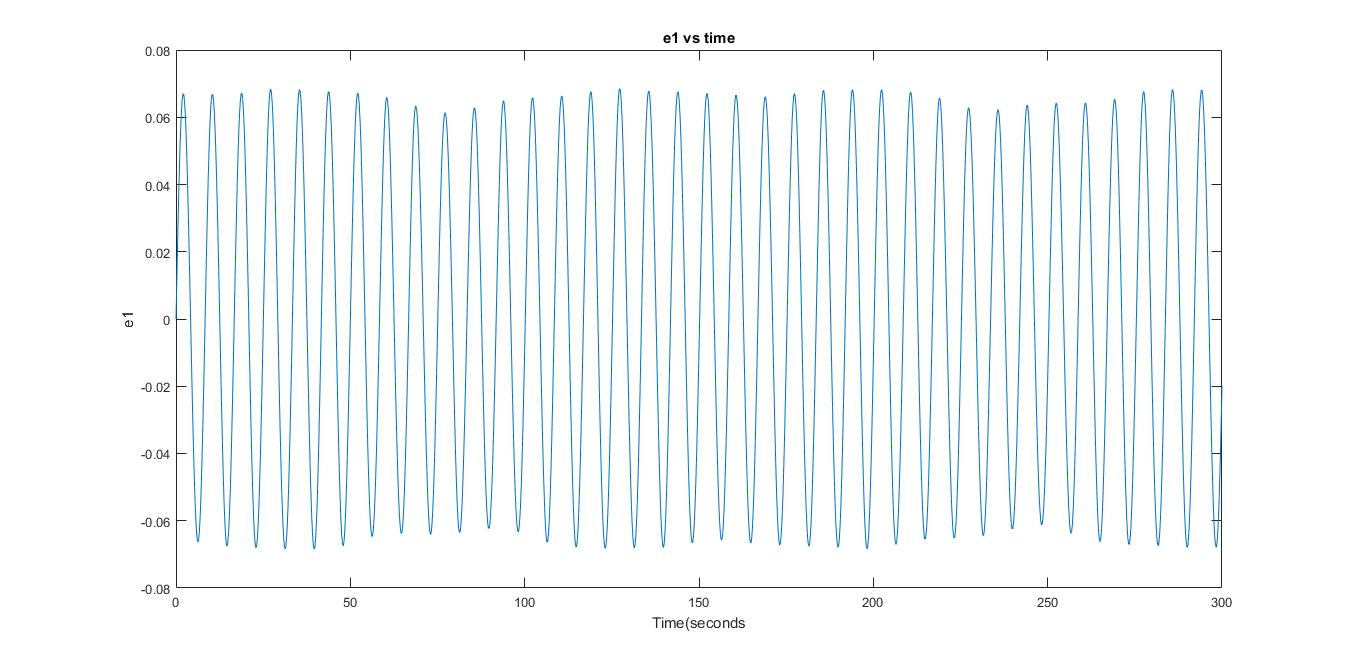
\includegraphics[scale=0.4]{spacecraft/e1}
\par\end{centering}
\caption{}
\end{figure}

\begin{figure}[H]
\begin{centering}
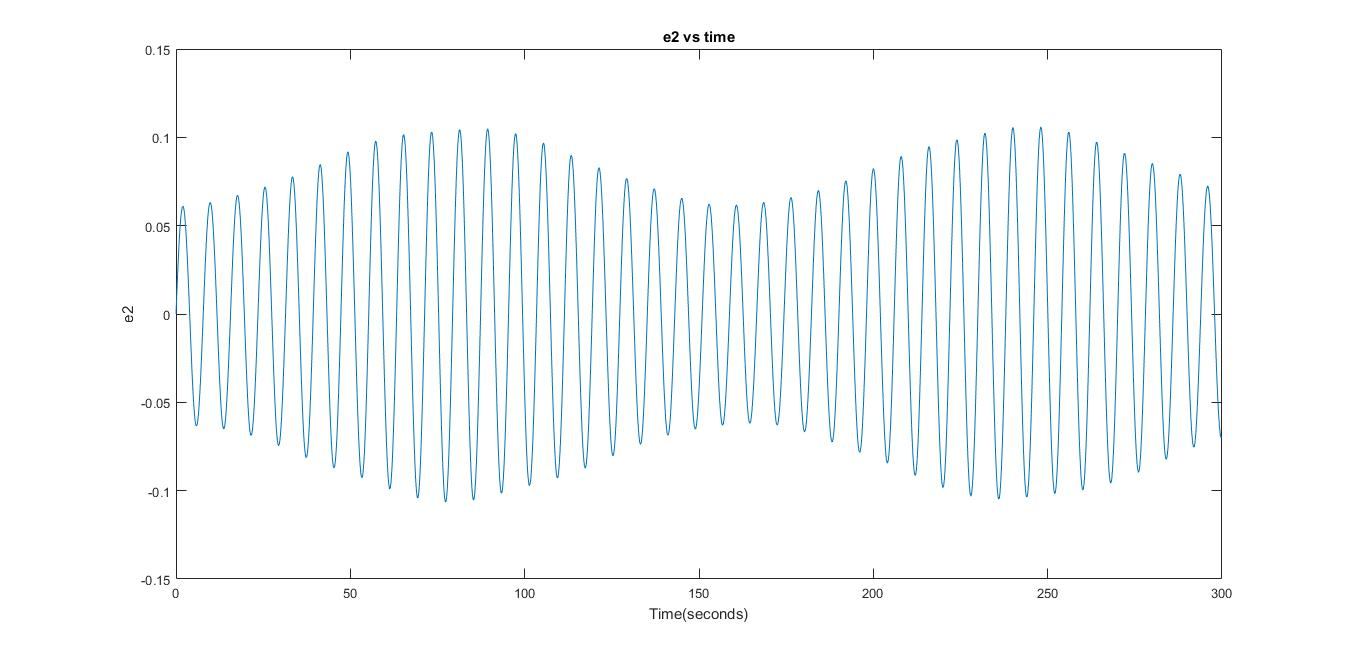
\includegraphics[scale=0.4]{spacecraft/e2}
\par\end{centering}
\caption{}
\end{figure}

\begin{figure}[H]
\begin{centering}
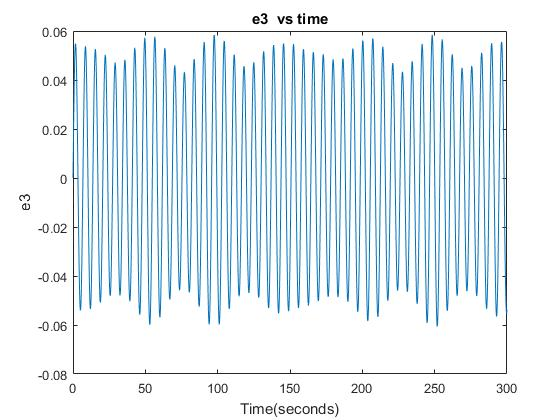
\includegraphics[scale=0.6]{spacecraft/e3}
\par\end{centering}
\caption{}
\end{figure}

\begin{figure}[H]
\begin{centering}
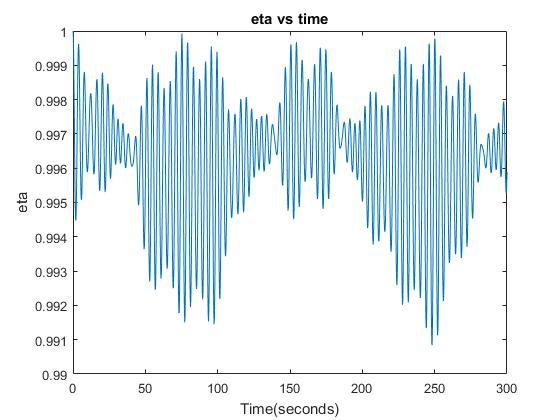
\includegraphics[scale=0.6]{spacecraft/eta}
\par\end{centering}
\caption{}
\end{figure}

The above plots show variation of quaternion in time without including
gravity gradient. It can be clearly seen they reach a stable value.

\textbf{Including Gravity gradient }

\noindent\begin{minipage}[t]{1\columnwidth}%
\begin{figure}[H]
\begin{centering}
\includegraphics[scale=0.4]{\string"results eps files/new/jpgs/Euler_angle_zero_ig_gg_wo_c\string".eps}
\par\end{centering}
\caption{}
\end{figure}

\begin{figure}[H]
\begin{centering}
\includegraphics[scale=0.4]{\string"results eps files/new/jpgs/Euler_rate_zero_ig_gg_wo_c\string".eps}
\par\end{centering}
\caption{}
\end{figure}
%
\end{minipage} 

\begin{figure}[H]
\begin{centering}
\includegraphics[scale=0.4]{\string"results eps files/new/jpgs/Euler_angle_zero_ig_gg_wo_c\string".eps}
\par\end{centering}
\caption{}
\end{figure}

\begin{figure}[H]
\begin{centering}
\includegraphics[scale=0.4]{\string"results eps files/new/jpgs/Euler_rate_zero_ig_gg_wo_c\string".eps}
\par\end{centering}
\caption{}
\end{figure}

As the gravity gradient torques are applied along with the given disturbances,
euler angles and rates both diverge with time as indicated by above
plots.

\begin{figure}[H]
\begin{centering}
\includegraphics[scale=0.4]{\string"results eps files/new/jpgs/Euler_angle_zero_ig_gg_w_c\string".eps}
\par\end{centering}
\caption{}
\end{figure}

\begin{figure}[H]
\begin{centering}
\includegraphics[scale=0.4]{\string"results eps files/new/jpgs/Euler_rate_zero_ig_gg_w_c\string".eps}
\par\end{centering}
\caption{}
\end{figure}

Even in the presence of gravity gradient torque and external disturbances,
the steady state errors of Euler angles and Rates are well within
0.005 deg and 0.005 deg/s.

\begin{figure}[H]
\begin{centering}
\includegraphics[scale=0.4]{\string"results eps files/new/jpgs/Wheel_1_torque_zero_ig_gg_w_c\string".eps}
\par\end{centering}
\caption{}
\end{figure}

\begin{figure}[H]
\begin{centering}
\includegraphics[scale=0.4]{\string"results eps files/new/jpgs/Wheel_2_torque_zero_ig_gg_w_c\string".eps}
\par\end{centering}
\caption{}
\end{figure}

\begin{figure}[H]
\begin{centering}
\includegraphics[scale=0.4]{\string"results eps files/new/jpgs/Wheel_3_torque_zero_ig_gg_w_c\string".eps}
\par\end{centering}
\caption{}
\end{figure}

\begin{figure}[H]
\begin{centering}
\includegraphics[scale=0.4]{\string"results eps files/new/jpgs/Wheel_4_torque_zero_ig_gg_w_c\string".eps}
\par\end{centering}
\caption{}
\end{figure}

From the above plots it is very clear that the torque level for none
of the wheels reached 0.5 Nm, hence there is no requirement of momentum
dumping even in the presence of gravity gradient torques and external
disturbances.

\section{Conclusion}

A modified PD controller was used to control Astrosat to make it stable
given a small disturbance. The gains $K_{p}$ and $K_{d}$ were set
so that the steady state errors in the euler angles do not exceed
0.005 degrees. Quaternions and momentum dumping strategies are also
addresed in this report apart from Euler angles approach.
\begin{thebibliography}{1}
\bibitem{key-1-1} Spacecraft Dynamics and Control - Marcel J.Sidis

\bibitem{key-1}Spacecraft Dynamics and Control - Anton de Ruiter,
Christopher Dameren, James Forbes
\end{thebibliography}

\end{document}
